\documentclass[11pt,letterpaper]{article}

% Packages
\usepackage[margin=1in]{geometry}
\usepackage{graphicx}
\usepackage{amsmath}
\usepackage{amssymb}
\usepackage{booktabs}
\usepackage{hyperref}
\usepackage{float}
\usepackage{caption}
\usepackage{subcaption}
\usepackage{fancyhdr}
\usepackage{titlesec}
\usepackage{enumitem}

% Header and footer
\pagestyle{fancy}
\fancyhf{}
\rhead{CS 5510 Homework 1}
\lhead{Benjamin Tran}
\rfoot{Page \thepage}

% Title formatting
\titleformat{\section}{\Large\bfseries}{\thesection}{1em}{}
\titleformat{\subsection}{\large\bfseries}{\thesubsection}{1em}{}

% Hyperref setup
\hypersetup{
    colorlinks=true,
    linkcolor=blue,
    filecolor=magenta,      
    urlcolor=cyan,
    citecolor=blue,
}

\begin{document}

% Title page
\begin{titlepage}
    \centering
    \vspace*{2cm}
    
    {\Huge\bfseries Reconstruction Attacks and Privacy Defenses\par}
    \vspace{0.5cm}
    {\Large An Empirical Study of Healthcare Data Privacy\par}
    \vspace{2cm}
    
    {\Large\itshape Benjamin Tran\par}
    \vspace{1cm}
    
    {\large CS 5510 - Data Privacy and Security\par}
    \vspace{0.5cm}
    {\large October 29, 2025\par}
    
    \vfill
    
    {\large \textbf{Abstract}\par}
    \vspace{0.5cm}
    \begin{minipage}{0.8\textwidth}
        \small
        This report investigates reconstruction attacks on sensitive healthcare data and evaluates three defense mechanisms: rounding, Gaussian noise, and subsampling. Using a synthetic dataset of 100 patient records, we demonstrate that reconstruction attacks can achieve 96.7\% accuracy with 200 queries when no defenses are employed. Our experimental analysis reveals that Gaussian noise provides the strongest protection with the best privacy-utility trade-off, transitioning at $\sigma = 2$. Rounding offers moderate protection at $R = 5$, while subsampling proves ineffective as a standalone defense. Additionally, we provide a Bayesian interpretation of Membership Inference Attacks, highlighting the critical importance of minimizing false positive rates for reliable inference.
    \end{minipage}
    
    \vfill
\end{titlepage}

\tableofcontents
\newpage

\section{Introduction}

The proliferation of data-driven healthcare systems has created unprecedented opportunities for medical research and personalized treatment. However, this data revolution also poses significant privacy risks. Even when sensitive attributes are not directly disclosed, adversaries can exploit statistical queries to reconstruct private information about individuals.

This report examines reconstruction attacks, which are a class of privacy attacks where an adversary uses multiple statistical queries to infer sensitive attributes of individuals in a dataset. We focus on a healthcare scenario where an attacker attempts to reconstruct medical test results (normal vs. abnormal) using only aggregate queries over public demographic attributes.

\subsection{Research Questions}

Our investigation addresses three primary questions:

\begin{enumerate}[leftmargin=*]
    \item \textbf{Attack Feasibility:} How accurately can an adversary reconstruct sensitive binary attributes using subset-sum queries?
    \item \textbf{Defense Effectiveness:} Which defense mechanisms (rounding, noise addition, or subsampling) effectively prevent reconstruction while maintaining data utility?
    \item \textbf{Privacy-Utility Trade-offs:} What are the optimal parameter settings that balance privacy protection with query accuracy?
\end{enumerate}

Additionally, we analyze Membership Inference Attacks (MIAs) from a Bayesian perspective to understand the role of false positive rates in privacy breaches.

\subsection{Contributions}

This work makes the following contributions:

\begin{itemize}[leftmargin=*]
    \item Comprehensive empirical evaluation of reconstruction attacks across 100 parameter settings per defense mechanism
    \item Identification of precise transition points where defenses become effective
    \item Comparative analysis revealing Gaussian noise as the optimal defense strategy
    \item Demonstration that subsampling alone is insufficient for privacy protection
    \item Bayesian framework for understanding membership inference attack reliability
\end{itemize}

\section{Background and Related Work}

\subsection{Reconstruction Attacks}

Reconstruction attacks exploit the fact that multiple statistical queries can leak information about individual records. When an adversary can issue many queries, they can construct a system of linear equations and solve for individual sensitive values. The feasibility of such attacks depends on:

\begin{itemize}[leftmargin=*]
    \item The number of queries allowed
    \item The diversity of query predicates
    \item The presence of noise or other defenses
\end{itemize}

\subsection{Defense Mechanisms}

Three primary defense strategies have been proposed:

\begin{enumerate}[leftmargin=*]
    \item \textbf{Output Perturbation:} Adding noise to query results (e.g., Laplace or Gaussian noise)
    \item \textbf{Rounding:} Discretizing query outputs to reduce information leakage
    \item \textbf{Input Perturbation:} Modifying the underlying dataset through sampling or generalization
\end{enumerate}

Our work evaluates representative mechanisms from each category in a controlled experimental setting.

\section{Methodology}

\subsection{Dataset Description}

We utilize a synthetic healthcare dataset containing 100 patient records. Each record consists of four public attributes and one sensitive binary attribute:

\textbf{Public Attributes} (known to the adversary):
\begin{itemize}[leftmargin=*]
    \item \texttt{age}: Patient age in years (range: 0--100)
    \item \texttt{sex}: Binary gender indicator (0 = male, 1 = female)
    \item \texttt{blood}: Blood type encoded as integers 0--7 representing A+, A-, B+, B-, AB+, AB-, O+, O-
    \item \texttt{admission}: Hospital admission type (0 = elective, 1 = urgent, 2 = emergency)
\end{itemize}

\textbf{Sensitive Attribute} (reconstruction target):
\begin{itemize}[leftmargin=*]
    \item \texttt{result}: Medical test outcome (0 = normal, 1 = abnormal)
\end{itemize}

The dataset contains 65 normal results (65\%) and 35 abnormal results (35\%), yielding a majority baseline accuracy of 0.650. This baseline serves as our threshold for attack success: reconstruction accuracy below 65\% indicates effective defense.

\subsubsection{Data and Code Sources}

The synthetic healthcare dataset used in this study was obtained from the OpenDP CS208 course repository\footnote{\url{https://github.com/opendp/cs208/blob/main/spring2025/data/fake_healthcare_dataset_sample100.csv}}. The initial implementation framework was adapted from the course's problem set starter code\footnote{\url{https://github.com/opendp/cs208/blob/main/spring2025/homeworks/ps2/ps2_starter.py}}, which was subsequently extended to include the defense mechanisms, experimental framework, and comprehensive evaluation metrics presented in this report.


\subsection{Attack Model}

The adversary has access to a query interface that computes subset-sum queries. For any boolean predicate $q$ defined over the public attributes, the interface returns:

\begin{equation}
    \text{Answer}(q) = \sum_{i: q(x_i) = \text{True}} \text{result}_i
\end{equation}

where $x_i$ represents the public attributes of patient $i$.

\subsubsection{Attack Strategy}

Our reconstruction attack proceeds as follows:

\begin{enumerate}[leftmargin=*]
    \item \textbf{Query Generation:} Generate 200 random boolean predicates over the public attributes (corresponding to $2n$ queries for $n=100$ patients)
    \item \textbf{Query Execution:} Submit each predicate to the query interface and collect responses
    \item \textbf{System Construction:} Formulate a system of linear equations $Ax = b$ where:
    \begin{itemize}
        \item $A$ is a $200 \times 100$ binary matrix (each row represents which patients satisfy a predicate)
        \item $x$ is the unknown $100$-dimensional sensitive attribute vector
        \item $b$ is the $200$-dimensional vector of query responses
    \end{itemize}
    \item \textbf{Optimization:} Solve the overdetermined system using least-squares optimization
    \item \textbf{Thresholding:} Round the continuous solution to binary values using threshold 0.5
\end{enumerate}

The implementation uses CPLEX optimization when available, falling back to standard least-squares regression otherwise.

\subsection{Defense Mechanisms}

We evaluate three defense mechanisms, each parameterized to allow fine-grained analysis of privacy-utility trade-offs.

\subsubsection{Defense 1: Rounding (Parameter $R$)}

Each query answer is rounded to the nearest multiple of $R$:

\begin{equation}
    \text{Answer}_{\text{defended}} = R \cdot \left\lfloor \frac{\text{Answer}_{\text{exact}}}{R} + 0.5 \right\rfloor
\end{equation}

\textbf{Conclusion:} Rounding reduces the precision of query answers, making it harder to distinguish between similar queries. Larger $R$ provides stronger privacy but introduces more distortion.

\subsubsection{Defense 2: Gaussian Noise (Parameter $\sigma$)}

Random noise sampled from $\mathcal{N}(0, \sigma^2)$ is added to each answer:

\begin{equation}
    \text{Answer}_{\text{defended}} = \text{Answer}_{\text{exact}} + \mathcal{N}(0, \sigma^2)
\end{equation}

\textbf{Conclusion:} Noise obscures the exact query result, introducing uncertainty that propagates through the reconstruction process. Larger $\sigma$ provides stronger privacy but reduces answer accuracy.

\subsubsection{Defense 3: Subsampling (Parameter $t$)}

A random subset of $t$ patients is sampled, the query is computed on this subset, and the result is scaled:

\begin{equation}
    \text{Answer}_{\text{defended}} = \frac{n}{t} \cdot \sum_{i \in S_t} \text{result}_i
\end{equation}

where $S_t$ is a uniformly random subset of size $t$.

\textbf{Conclusion:} Subsampling introduces variance by computing on incomplete data. Smaller $t$ provides stronger privacy but increases variance dramatically.

\subsection{Experimental Design}

\subsubsection{Parameter Ranges}

To comprehensively evaluate each defense, we test the full range of integer parameters from 1 to 100:

\begin{itemize}[leftmargin=*]
    \item \textbf{Rounding:} $R \in \{1, 2, 3, \ldots, 100\}$
    \item \textbf{Gaussian Noise:} $\sigma \in \{1, 2, 3, \ldots, 100\}$
    \item \textbf{Subsampling:} $t \in \{1, 2, 3, \ldots, 100\}$
\end{itemize}

\subsubsection{Evaluation Protocol}

For each defense and parameter value:

\begin{enumerate}[leftmargin=*]
    \item Run 10 independent trials with different random seeds
    \item Generate 200 fresh random predicates per trial
    \item Execute the reconstruction attack
    \item Compute evaluation metrics
\end{enumerate}

\subsubsection{Evaluation Metrics}

We measure both utility (query accuracy) and privacy (reconstruction difficulty):

\begin{itemize}[leftmargin=*]
    \item \textbf{Root Mean Squared Error (RMSE):} Measures the average distortion between defended and exact query answers:
    \begin{equation}
        \text{RMSE} = \sqrt{\frac{1}{m} \sum_{j=1}^{m} (\text{Answer}_{\text{defended}}^{(j)} - \text{Answer}_{\text{exact}}^{(j)})^2}
    \end{equation}
    where $m = 200$ is the number of queries.
    
    \item \textbf{Success Rate:} Fraction of correctly reconstructed sensitive values:
    \begin{equation}
        \text{Success Rate} = \frac{1}{n} \sum_{i=1}^{n} \mathbb{1}[\text{predicted}_i = \text{actual}_i]
    \end{equation}
    
    \item \textbf{Transition Point:} The smallest parameter value where success rate falls below the majority baseline (0.650)
\end{itemize}

\section{Results}

\subsection{Baseline Attack Performance}

Without any defenses, the reconstruction attack achieves great accuracy:

\begin{itemize}[leftmargin=*]
    \item \textbf{Success Rate:} 96.7\% (97 out of 100 sensitive values correctly reconstructed)
    \item \textbf{Exact Reconstruction:} Achieved in multiple trials
    \item \textbf{RMSE:} 0.00 (queries return exact values)
\end{itemize}

This demonstrates the severe privacy risk posed by unrestricted statistical queries, even when only aggregate information is released.

\subsection{Defense 1: Rounding}

Table~\ref{tab:rounding} summarizes the performance of the rounding defense across key parameter values.

\begin{table}[H]
\centering
\caption{Rounding Defense Performance}
\label{tab:rounding}
\begin{tabular}{@{}cccc@{}}
\toprule
\textbf{Parameter $R$} & \textbf{RMSE} & \textbf{Success Rate} & \textbf{Status} \\ \midrule
1 & 0.00 & 0.967 & Attack succeeds \\
2 & 0.65 & 0.733 & Attack succeeds \\
3 & 0.76 & 0.688 & Attack succeeds \\
4 & 1.10 & 0.666 & Attack succeeds \\
\textbf{5} & \textbf{1.20} & \textbf{0.606} & \textbf{Attack fails} \\
6 & 1.56 & 0.584 & Attack fails \\
8 & 2.16 & 0.570 & Attack fails \\
10 & 2.62 & 0.585 & Attack fails \\ \bottomrule
\end{tabular}
\end{table}

\textbf{Key Findings:}

\begin{itemize}[leftmargin=*]
    \item \textbf{Transition Point:} $R = 5$ is the critical threshold where reconstruction success drops to 60.6\%, falling below the majority baseline
    \item \textbf{Sharp Transition:} Success rate drops from 66.6\% at $R=4$ to 60.6\% at $R=5$, indicating a relatively sharp phase transition
    \item \textbf{Utility Cost:} At the transition point, RMSE is only 1.20, representing minimal distortion
    \item \textbf{Discrete Behavior:} Both RMSE and success rate exhibit step-like patterns due to the discrete nature of rounding
\end{itemize}

\textbf{Interpretation:} Rounding provides moderate privacy protection with predictable utility degradation. The defense becomes effective at relatively small parameter values, making it practical for scenarios requiring deterministic query answers.

\subsection{Defense 2: Gaussian Noise}

Table~\ref{tab:noise} presents the performance of the Gaussian noise defense.

\begin{table}[H]
\centering
\caption{Gaussian Noise Defense Performance}
\label{tab:noise}
\begin{tabular}{@{}cccc@{}}
\toprule
\textbf{Parameter $\sigma$} & \textbf{RMSE} & \textbf{Success Rate} & \textbf{Status} \\ \midrule
1 & 1.02 & 0.653 & Attack succeeds \\
\textbf{2} & \textbf{1.99} & \textbf{0.598} & \textbf{Attack fails} \\
3 & 3.03 & 0.545 & Attack fails \\
4 & 4.06 & 0.534 & Attack fails \\
5 & 5.02 & 0.524 & Attack fails \\
6 & 5.88 & 0.519 & Attack fails \\
8 & 8.11 & 0.519 & Attack fails \\
10 & 10.34 & 0.526 & Attack fails \\ \bottomrule
\end{tabular}
\end{table}

\textbf{Key Findings:}

\begin{itemize}[leftmargin=*]
    \item \textbf{Transition Point:} $\sigma = 2$ provides effective protection, with success dropping to 59.8\%
    \item \textbf{Sharpest Transition:} The defense exhibits the most extreme phase transition among all three mechanisms
    \item \textbf{Excellent Trade-off:} At $\sigma = 2$, RMSE is only 1.99 while providing strong privacy protection
    \item \textbf{Linear RMSE Growth:} RMSE increases approximately linearly with $\sigma$, making utility costs predictable
    \item \textbf{Diminishing Returns:} Success rate plateaus around 51\% for large $\sigma$, suggesting fundamental limits
\end{itemize}

\textbf{Interpretation:} Gaussian noise emerges as the most effective defense, offering the best privacy-utility trade-off. Even minimal noise ($\sigma = 2$) significantly degrades attack performance while maintaining reasonable query accuracy.

\subsection{Defense 3: Subsampling}

Table~\ref{tab:subsampling} shows the performance of the subsampling defense.

\begin{table}[H]
\centering
\caption{Subsampling Defense Performance}
\label{tab:subsampling}
\begin{tabular}{@{}cccc@{}}
\toprule
\textbf{Parameter $t$} & \textbf{RMSE} & \textbf{Success Rate} & \textbf{Status} \\ \midrule
1 & 21.88 & 0.647 & Attack succeeds \\
6 & 12.89 & 0.556 & Attack fails \\
11 & 10.09 & 0.576 & Attack fails \\
21 & 6.72 & 0.593 & Attack fails \\
51 & 3.58 & 0.740 & Attack succeeds \\
71 & 2.35 & 0.824 & Attack succeeds \\
81 & 1.71 & 0.876 & Attack succeeds \\
91 & 1.00 & 0.944 & Attack succeeds \\
\textbf{96} & \textbf{0.72} & \textbf{0.975} & \textbf{No defense} \\ \bottomrule
\end{tabular}
\end{table}

\textbf{Key Findings:}

\begin{itemize}[leftmargin=*]
    \item \textbf{Paradoxical Behavior:} Subsampling shows effective protection for small $t$ values ($t \leq 21$), with success rates below the 65\% baseline
    \item \textbf{Success Rate Increases with $t$:} As $t$ increases, success rate rises from 64.7\% at $t=1$ to 97.5\% at $t=96$
    \item \textbf{Extreme Utility Cost:} Small $t$ values produce massive RMSE (21.88 at $t=1$), making the data nearly unusable despite providing privacy
    \item \textbf{Poor Privacy-Utility Trade-off:} Cannot achieve both good privacy and good utility simultaneously---must choose one or the other
\end{itemize}

\textbf{Interpretation:} Subsampling exhibits a paradoxical privacy-utility trade-off. While small $t$ values (e.g., $t \leq 21$) do prevent reconstruction (success below baseline), they introduce catastrophic variance (RMSE $> 6$), making query answers unreliable for practical use. Larger $t$ values provide acceptable utility but offer no privacy protection. Unlike noise and rounding, subsampling cannot achieve meaningful privacy with acceptable utility simultaneously.

\subsection{Comparative Analysis}

The following sections provide a comprehensive comparison of all three defense mechanisms based on their effectiveness, privacy-utility trade-offs, and practical applicability.

\subsubsection{Defense Effectiveness Ranking}

\begin{enumerate}[leftmargin=*]
    \item \textbf{Gaussian Noise} ($\sigma^* = 2$): Strongest protection with best trade-off. Success drops to 59.8\%, RMSE = 1.99
    \item \textbf{Rounding} ($R^* = 5$): Moderate protection with excellent utility. Success drops to 60.6\%, RMSE = 1.20
    \item \textbf{Subsampling}: Technically can provide protection (at $t \leq 21$: success below 65\% baseline) but at catastrophic utility cost (RMSE = 6.72 at $t=21$). No practical parameter value achieves both privacy and utility
\end{enumerate}

\subsubsection{Privacy-Utility Trade-offs}

\begin{itemize}[leftmargin=*]
    \item \textbf{Rounding:} Offers the best utility (lowest RMSE = 1.20) at the transition point, but provides weaker privacy than noise
    \item \textbf{Gaussian Noise:} Provides the strongest privacy with acceptable utility cost (RMSE = 1.99)
    \item \textbf{Subsampling:} Can provide privacy but only at unacceptable utility costs. Exhibits poor trade-off where privacy and utility cannot both be satisfied
\end{itemize}

Figure~\ref{fig:tradeoff_comparison} illustrates the privacy-utility trade-offs for all three defense mechanisms, showing the relationship between reconstruction success rate (privacy) and RMSE (utility) across different parameter values.

\begin{figure}[H]
    \centering
    \begin{subfigure}[b]{0.45\textwidth}
        \centering
        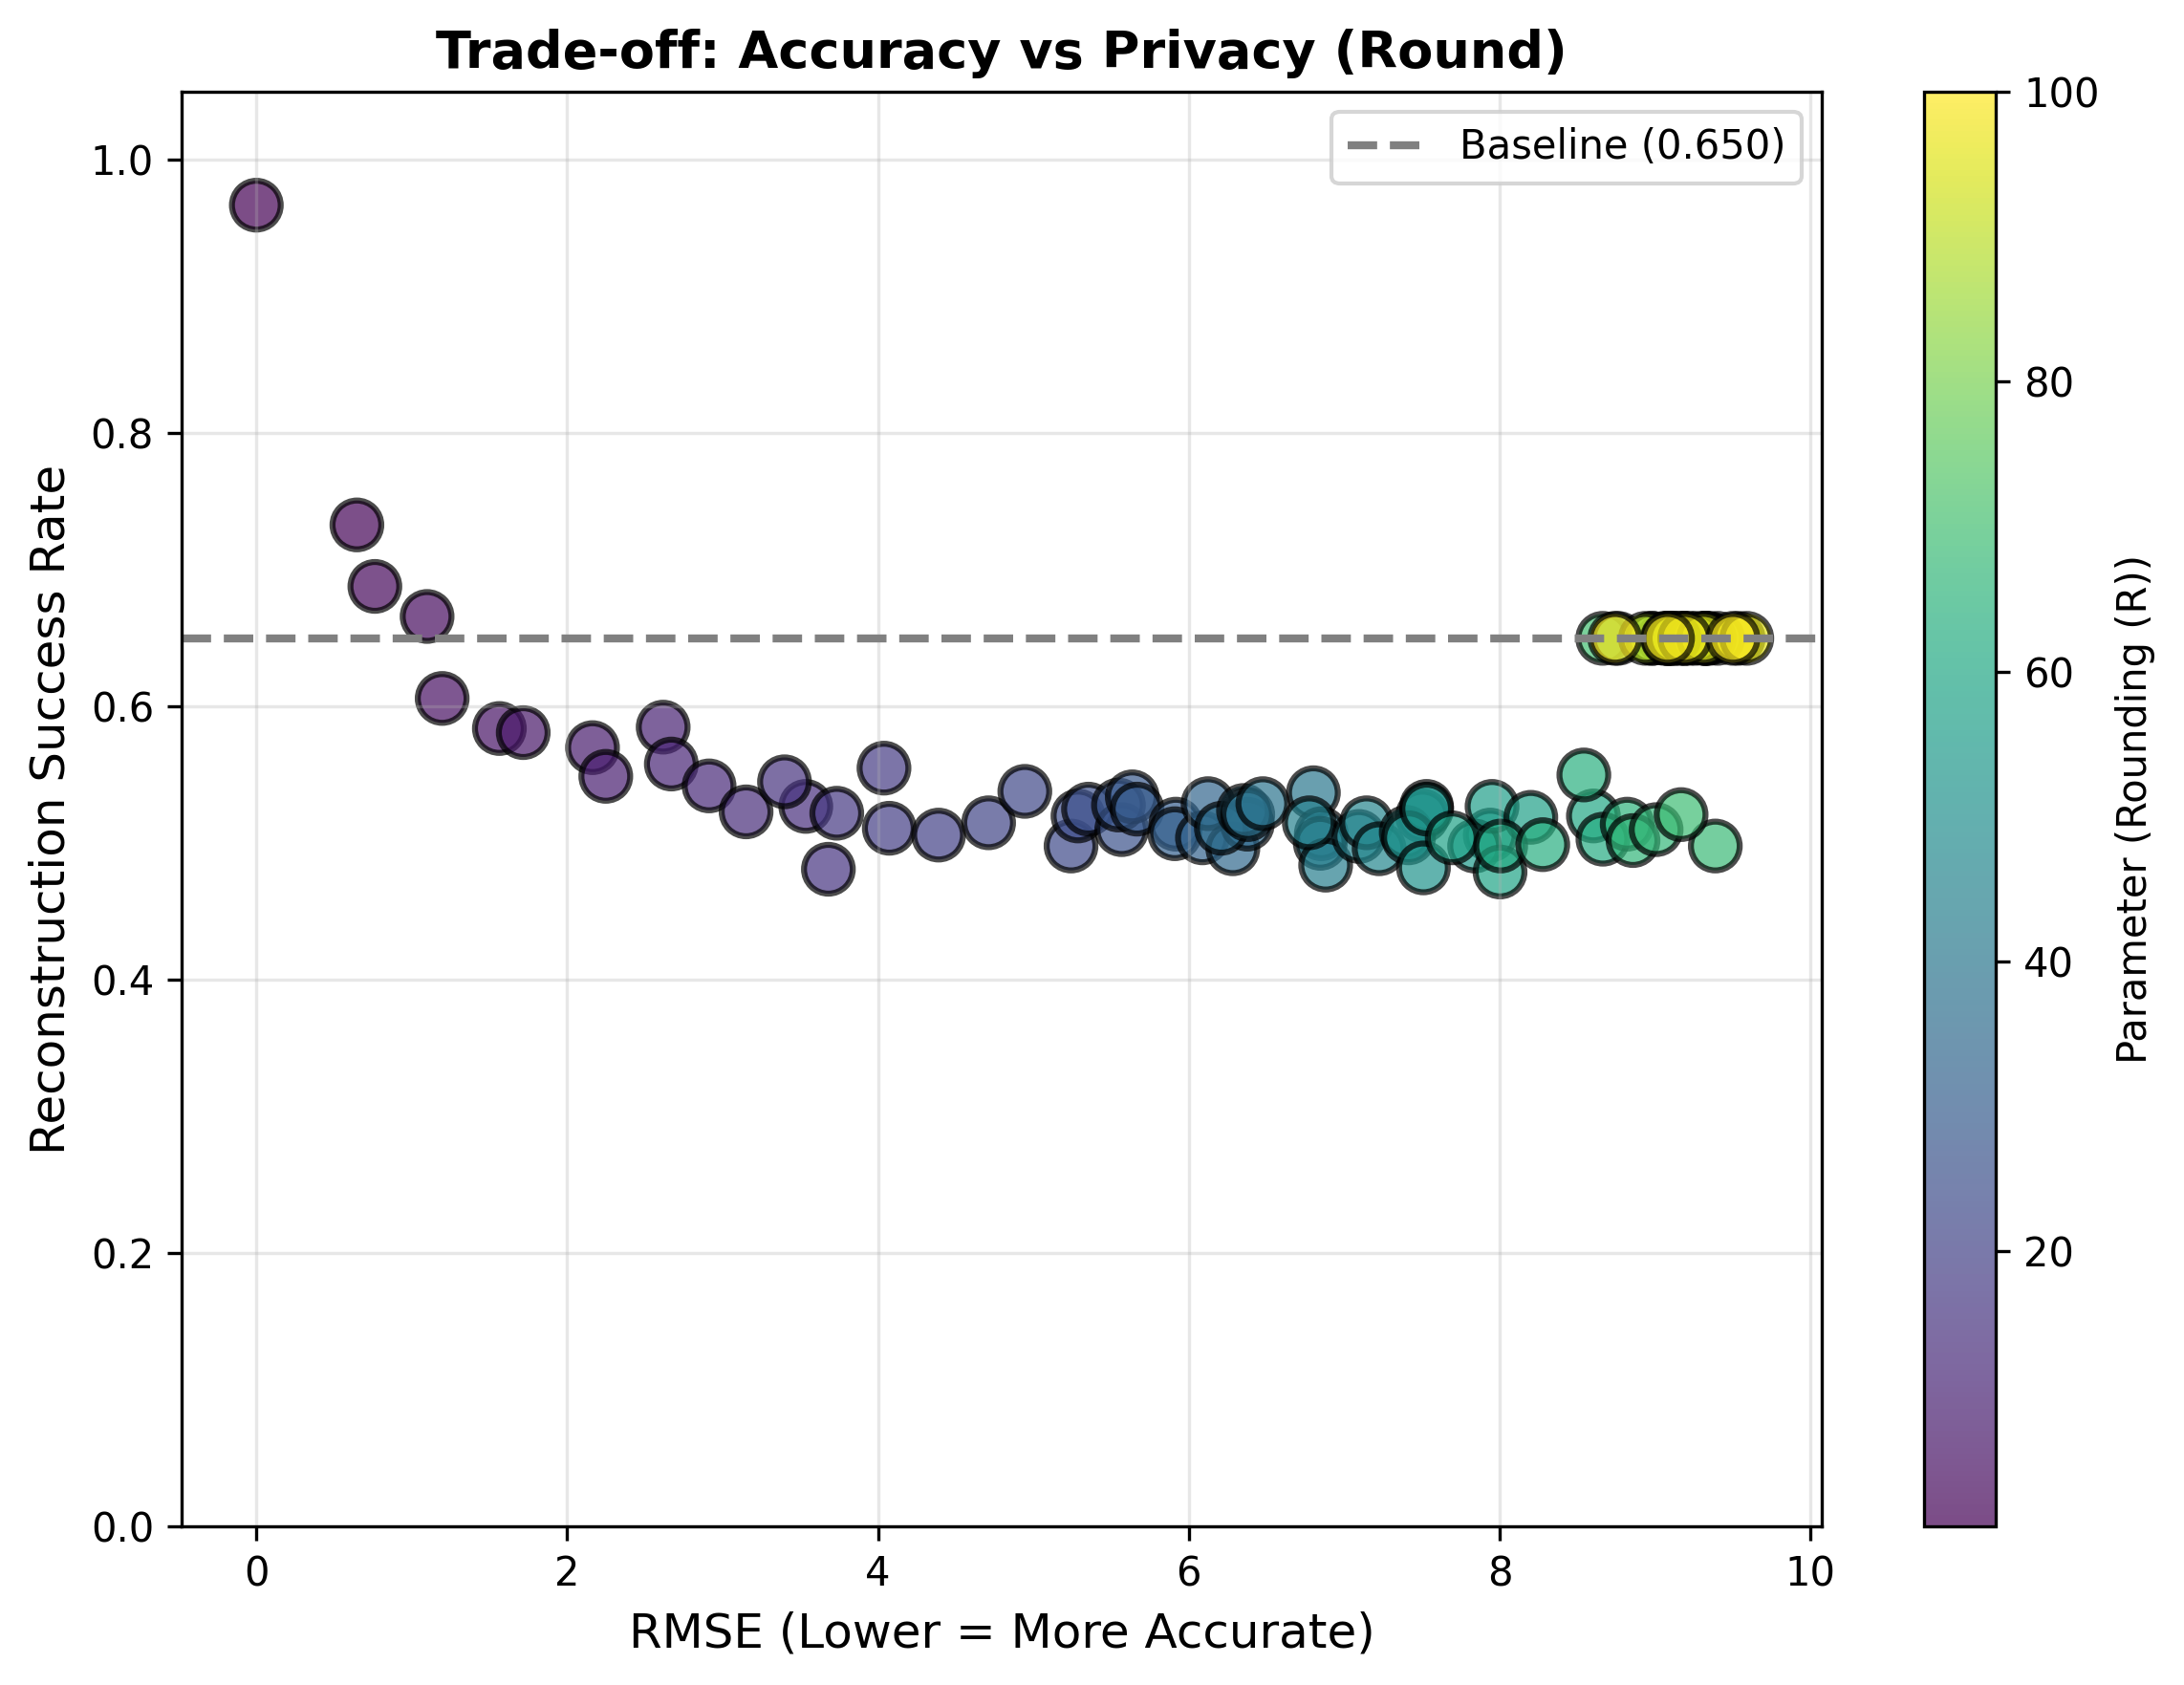
\includegraphics[width=\textwidth]{tradeoff_round.png}
        \caption{Rounding}
    \end{subfigure}
    \hfill
    \begin{subfigure}[b]{0.45\textwidth}
        \centering
        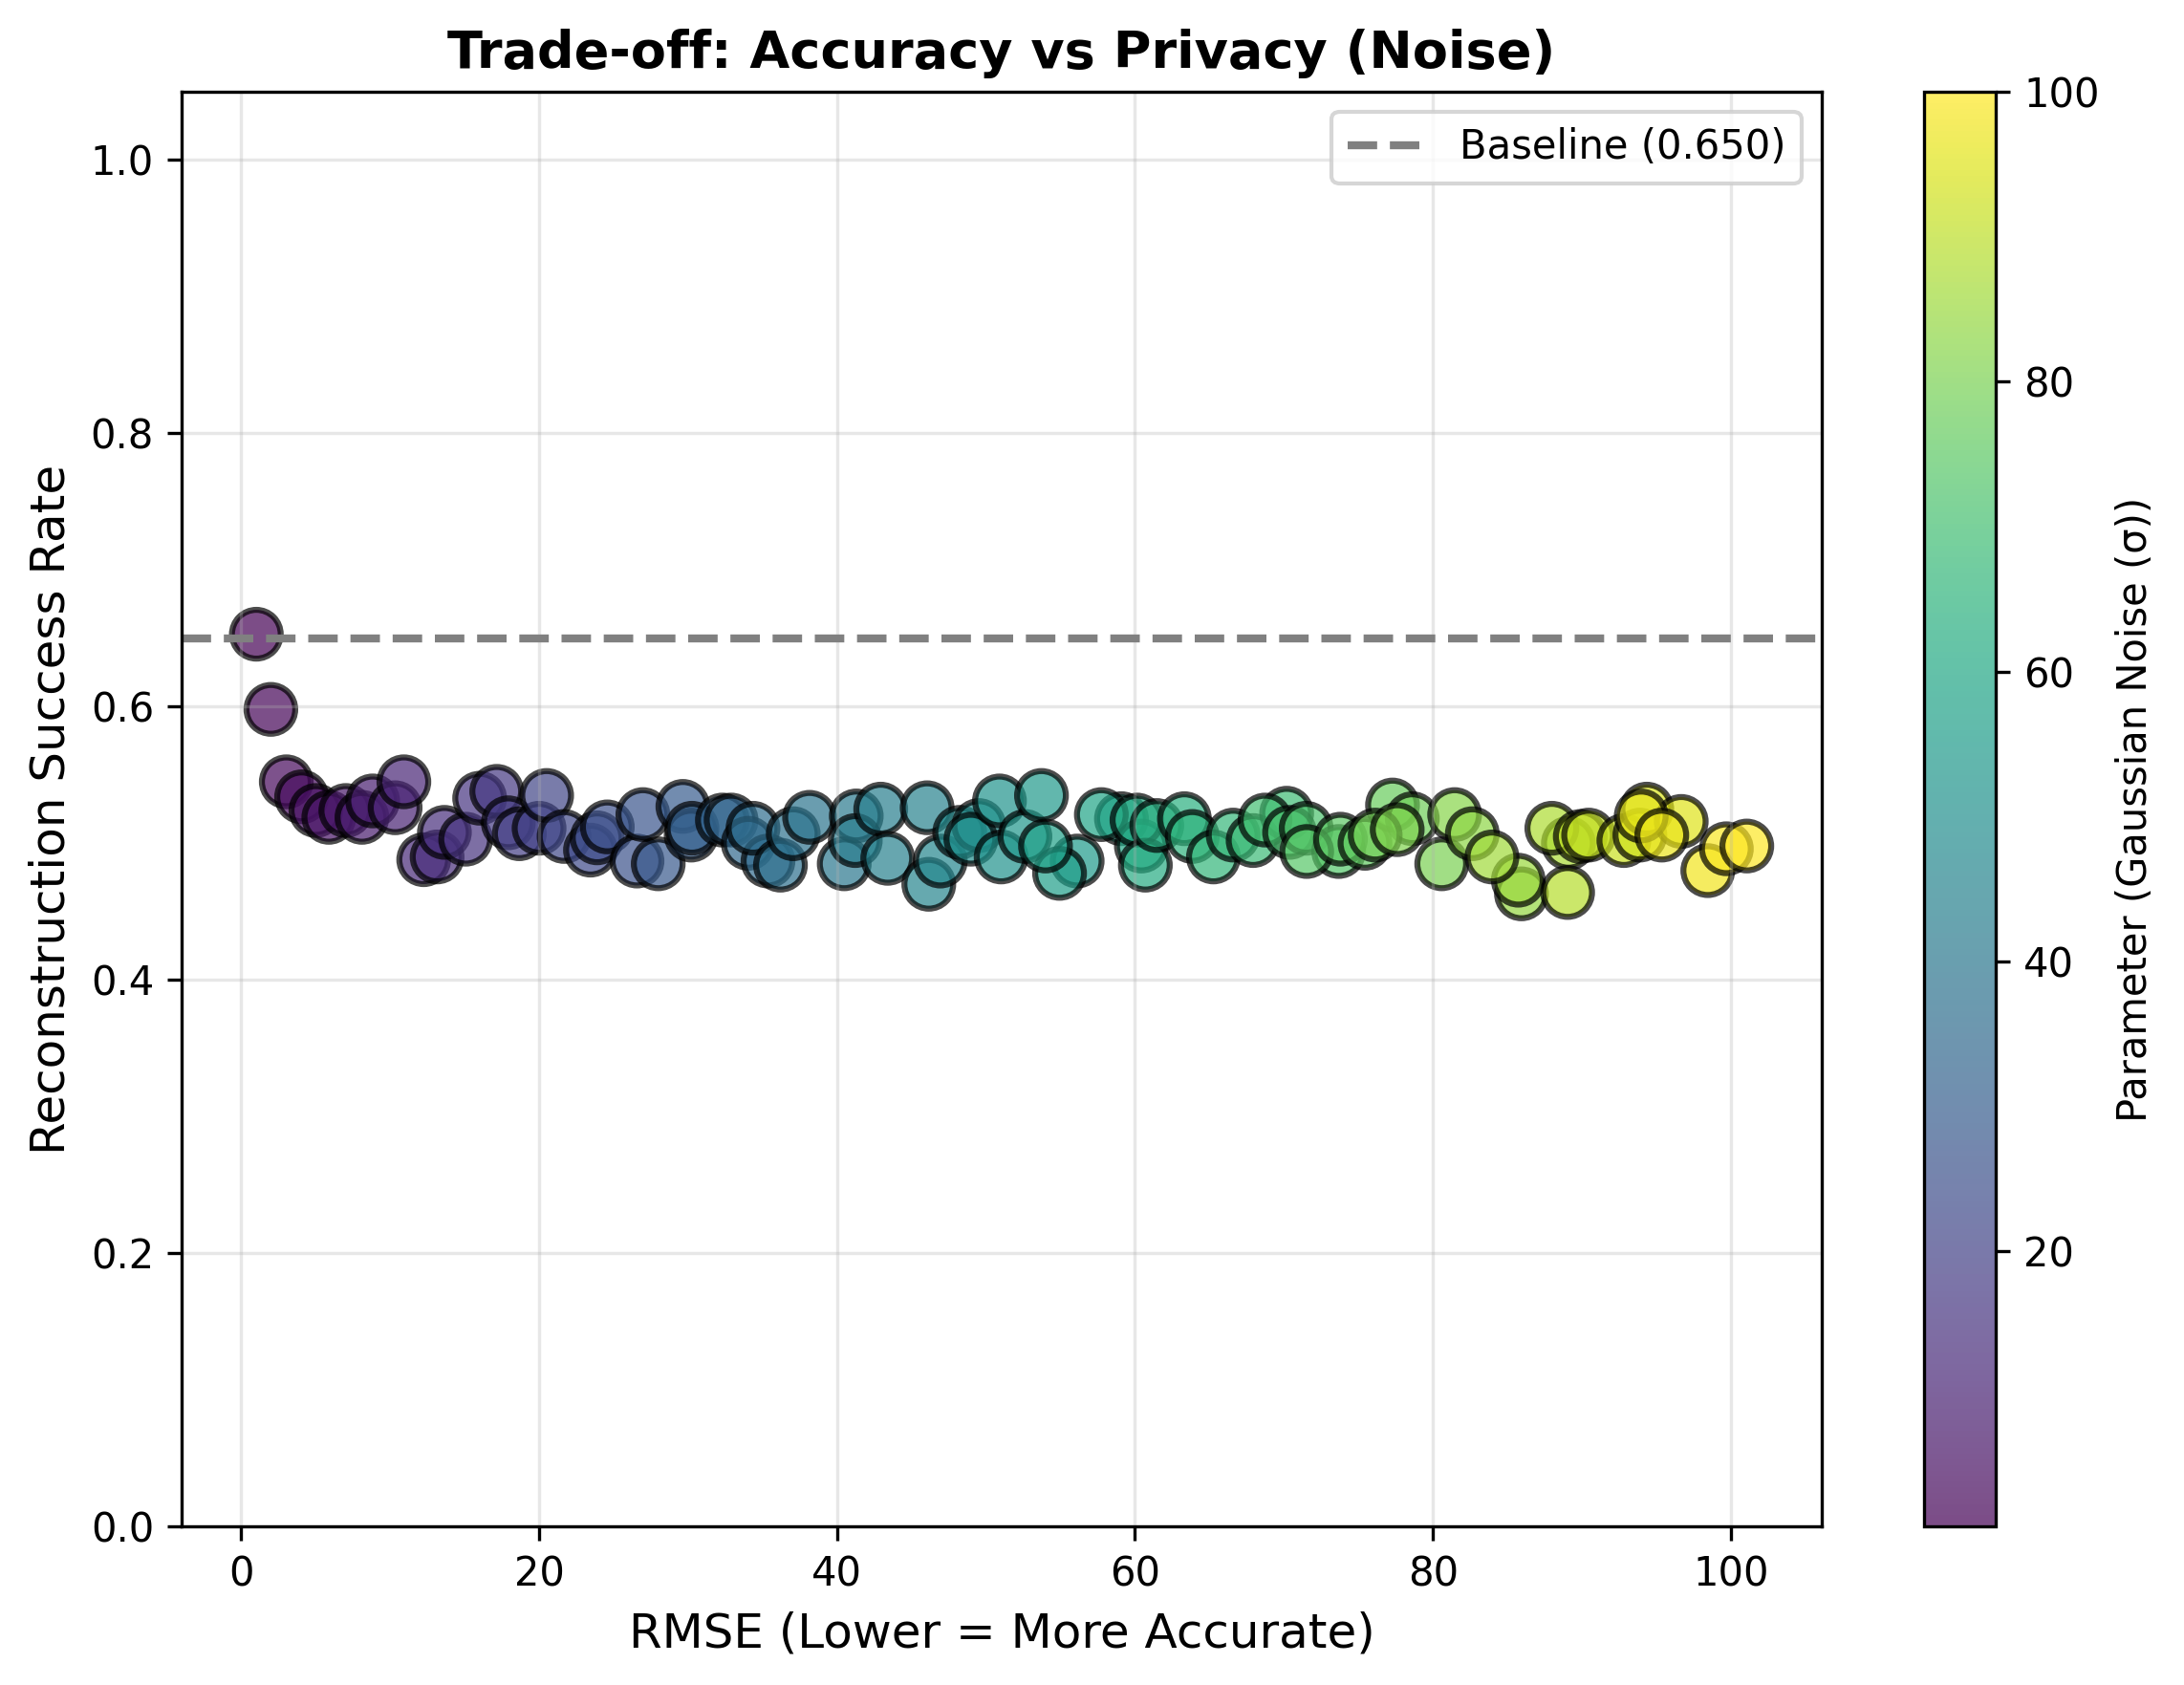
\includegraphics[width=\textwidth]{tradeoff_noise.png}
        \caption{Gaussian Noise}
    \end{subfigure}
    \hfill
    \begin{subfigure}[b]{0.45\textwidth}
        \centering
        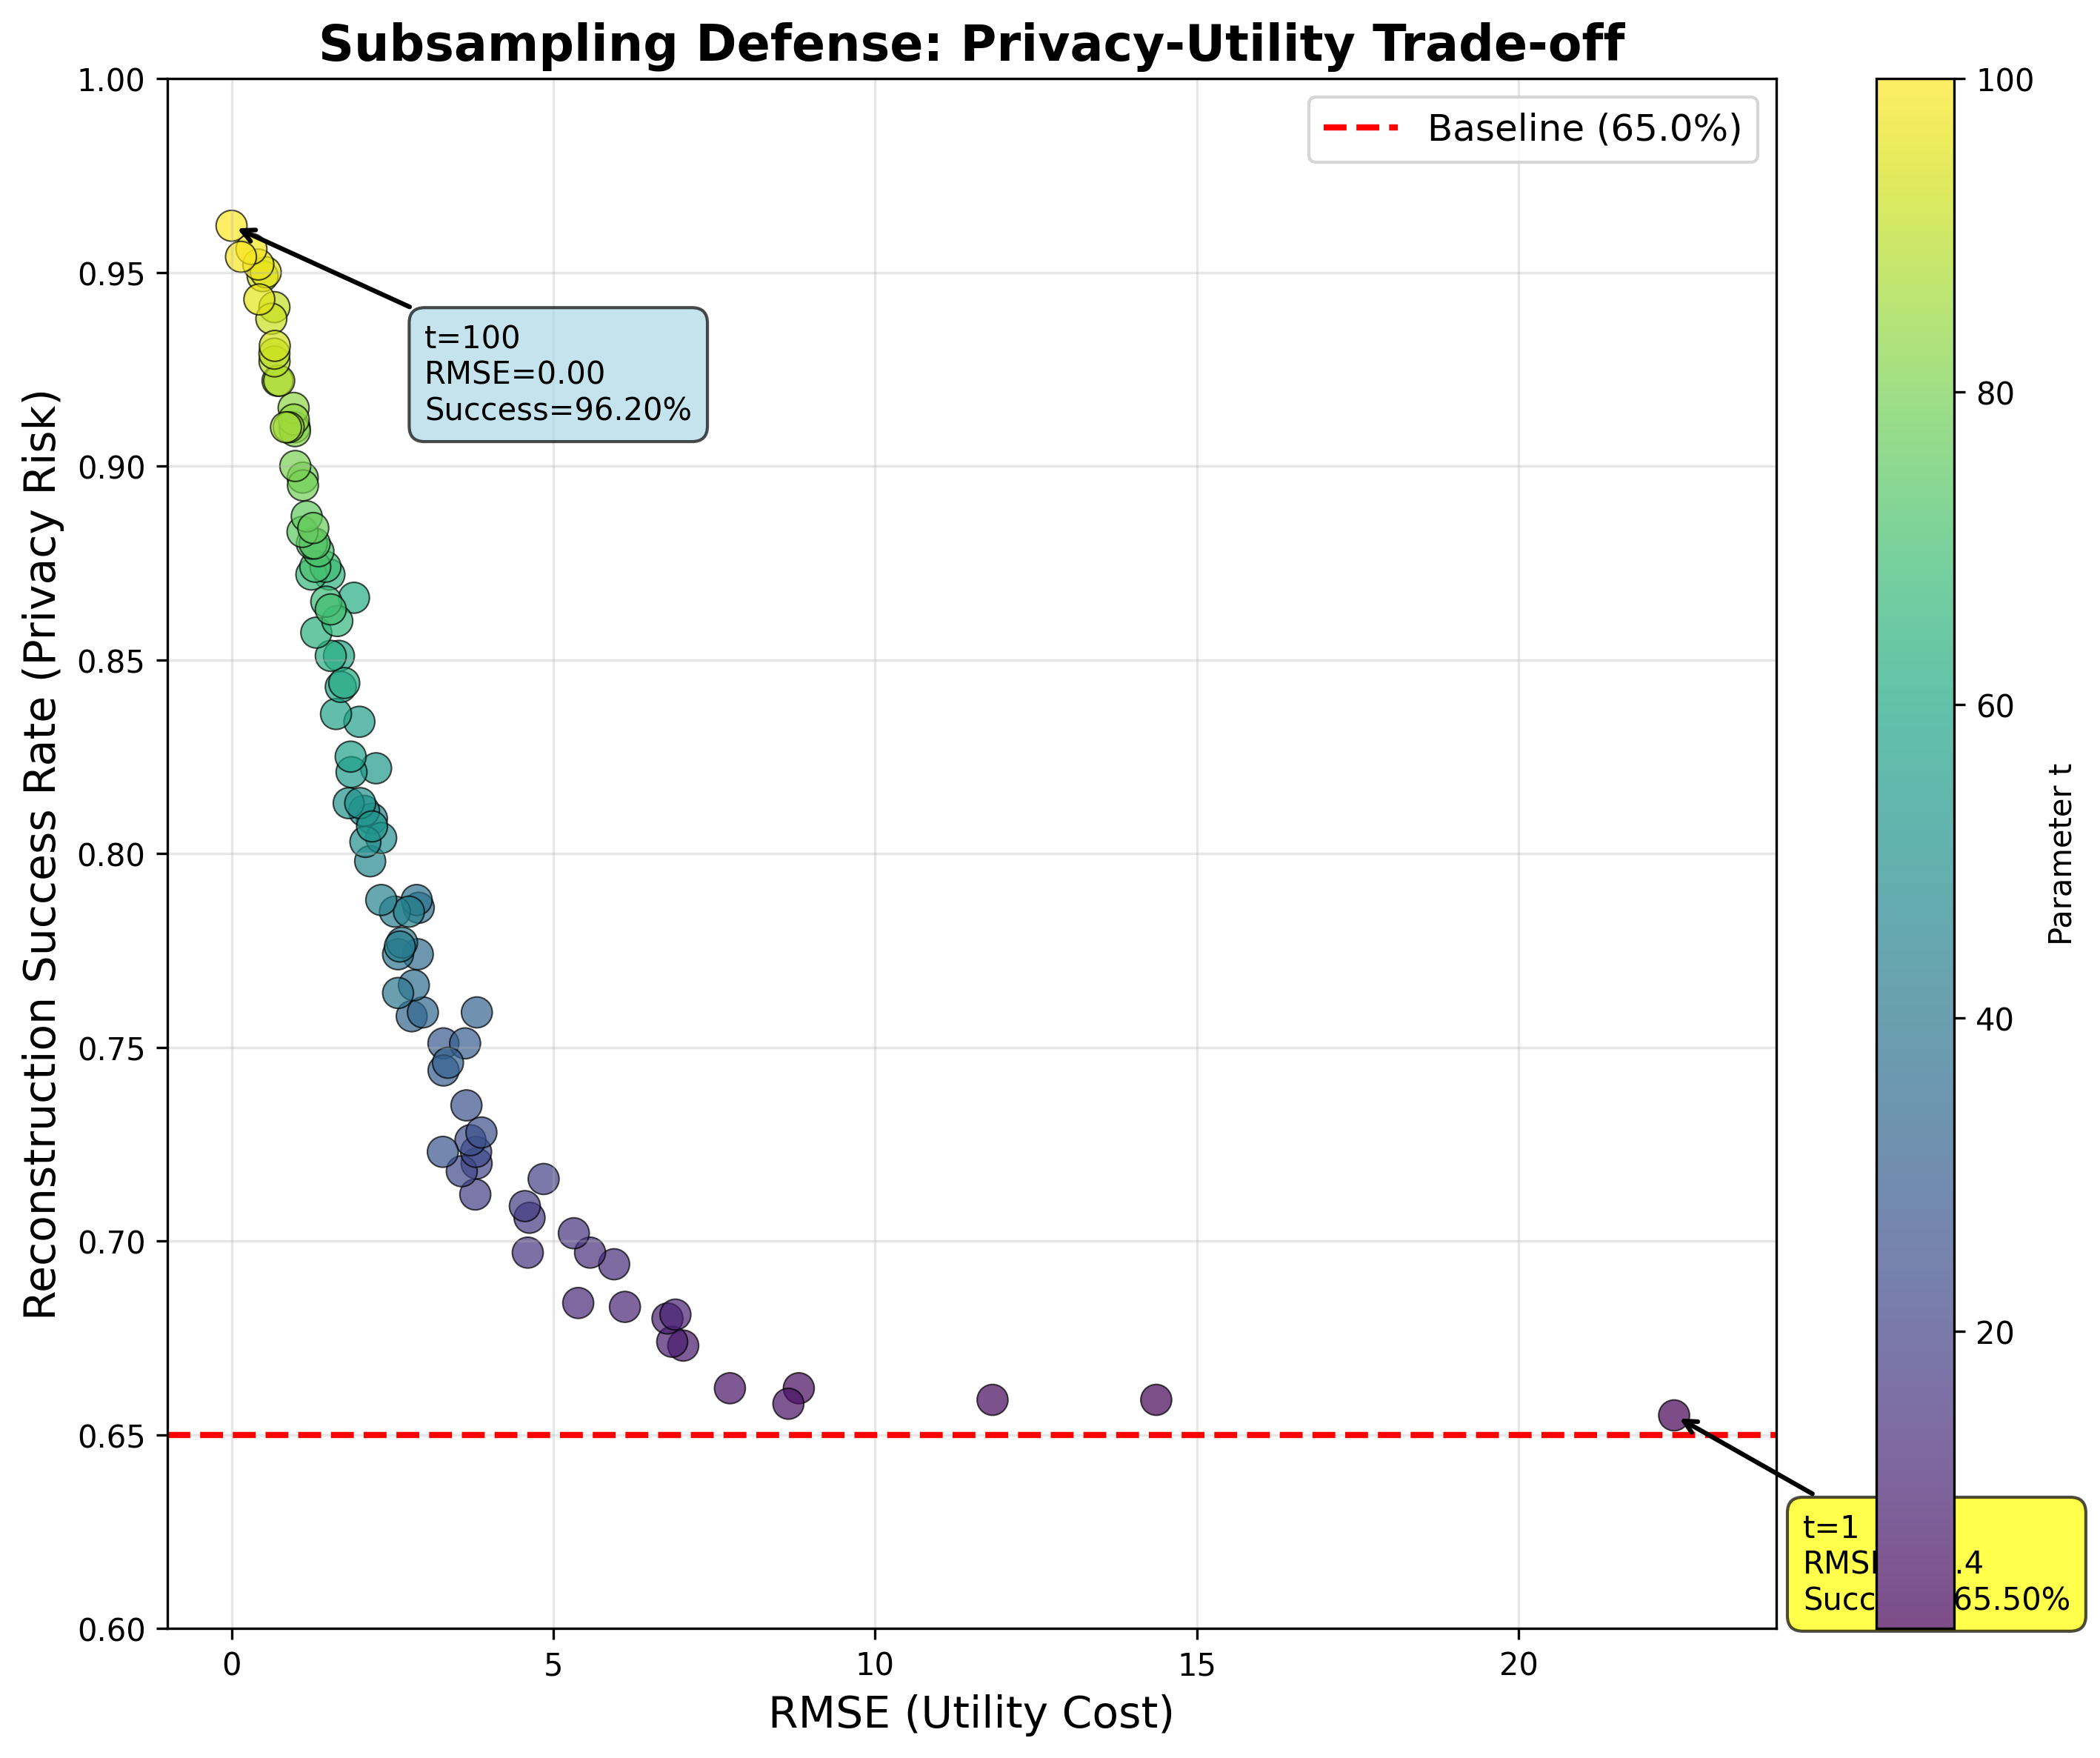
\includegraphics[width=\textwidth]{tradeoff_sample.png}
        \caption{Subsampling}
    \end{subfigure}
    \caption{Privacy-Utility Trade-offs: Comparison of all three defense mechanisms showing success rate vs. RMSE. Lower success rates and lower RMSE values are desirable (bottom-left corner). Gaussian noise provides the best trade-off, while subsampling fails to provide meaningful privacy protection.}
    \label{fig:tradeoff_comparison}
\end{figure}

\subsubsection{Practical Recommendations}

Based on our empirical findings:

\begin{itemize}[leftmargin=*]
    \item \textbf{Recommended:} Use Gaussian noise with $\sigma \geq 2$ for effective privacy protection with minimal utility loss (RMSE $\approx$ 2)
    \item \textbf{Alternative:} Use rounding with $R \geq 5$ when deterministic answers are required, offering slightly better utility (RMSE $\approx$ 1.2)
    \item \textbf{Avoid:} Do not use subsampling as a standalone privacy defense. While it can technically prevent attacks at small $t$, the utility cost (RMSE $> 6$) makes the data practically unusable
\end{itemize}

\section{Bayesian Interpretation of Membership Inference Attacks}

Beyond reconstruction attacks, we analyze Membership Inference Attacks (MIAs) through a Bayesian lens to understand when such attacks provide reliable evidence of membership.

\subsection{Problem}

Consider an attacker who believes that an individual Alice is in a dataset with prior probability $p$. We express this belief as prior odds:

\begin{equation}
    O_{\text{prior}} = \frac{p}{1-p}
\end{equation}

An MIA algorithm examines the dataset and outputs either ``In'' or ``Out''. The algorithm is characterized by:

\begin{itemize}[leftmargin=*]
    \item \textbf{True Positive Rate (TPR):} $P(\text{MIA says ``In''} \mid \text{Alice actually in})$
    \item \textbf{False Positive Rate (FPR):} $P(\text{MIA says ``In''} \mid \text{Alice actually out})$
\end{itemize}

\textbf{Question:} If the MIA returns ``In'', what are the posterior odds $O_{\text{post}}$ that Alice is actually in the dataset?

\subsection{Derivation}

Using Bayes' theorem, we compute the posterior odds:

\begin{align}
    O_{\text{post}} &= \frac{P(\text{In} \mid \text{``In''})}{P(\text{Out} \mid \text{``In''})} \\
    &= \frac{P(\text{``In''} \mid \text{In}) \cdot P(\text{In})}{P(\text{``In''} \mid \text{Out}) \cdot P(\text{Out})} \\
    &= \frac{\text{TPR} \cdot p}{\text{FPR} \cdot (1-p)} \\
    &= \frac{\text{TPR}}{\text{FPR}} \cdot \frac{p}{1-p}
\end{align}

Therefore:

\begin{equation}
    \boxed{O_{\text{post}} = \frac{\text{TPR}}{\text{FPR}} \cdot O_{\text{prior}}}
\end{equation}

The ratio $\text{TPR}/\text{FPR}$ is called the \textbf{likelihood ratio} and quantifies how much evidence the MIA provides.

\subsection{Significance of Small False Positive Rate}

The likelihood ratio reveals why minimizing FPR is critical for reliable membership inference, even when TPR is high.

\subsubsection{Example 1: Large FPR (Weak Evidence)}

Consider an MIA with perfect detection but poor specificity:
\begin{itemize}[leftmargin=*]
    \item TPR = 1.0 (detects all members)
    \item FPR = 0.5 (50\% false positive rate)
    \item Likelihood ratio = $1.0 / 0.5 = 2$
\end{itemize}

A positive result only \textit{doubles} our prior belief. If we initially believed Alice had a 10\% chance of membership ($O_{\text{prior}} = 0.111$), the posterior odds become $O_{\text{post}} = 0.222$, corresponding to only 18\% probability, which is unlikely.

\subsubsection{Example 2: Small FPR (Strong Evidence)}

Now consider an MIA with excellent specificity:
\begin{itemize}[leftmargin=*]
    \item TPR = 1.0 (detects all members)
    \item FPR = 0.01 (1\% false positive rate)
    \item Likelihood ratio = $1.0 / 0.01 = 100$
\end{itemize}

A positive result multiplies our belief by 100! With the same 10\% prior, the posterior odds become $O_{\text{post}} = 11.1$, corresponding to 91\% probability, which is a very strong evidence of membership.

\subsubsection{Conclusion}

A small FPR is important because:

\begin{enumerate}[leftmargin=*]
    \item It makes the likelihood ratio large, providing strong evidence when the MIA claims membership
    \item With large FPR, many false positives occur, making positive results unreliable
    \item High TPR alone is insufficient, because specificity (low FPR) determines the evidential value
    \item This explains why differential privacy mechanisms focus on limiting distinguishability (related to FPR control)
\end{enumerate}

\section{Discussion}

\subsection{Implications for Privacy Protection}

Our results demonstrate that reconstruction attacks pose a serious threat to privacy in systems that release aggregate statistics. Even with 200 queries on a dataset of 100 individuals, an adversary can reconstruct 96.7\% of sensitive values without any defenses.

The effectiveness of defenses varies:

\begin{itemize}[leftmargin=*]
    \item \textbf{Gaussian noise} provides strong protection with minimal utility loss, making it the preferred choice for most applications
    \item \textbf{Rounding} offers an alternative with slightly better utility but weaker privacy
    \item \textbf{Subsampling} is ineffective as a standalone defense and should not be relied upon for privacy protection
\end{itemize}

\subsection{Limitations}

Our study has several limitations:

\begin{enumerate}[leftmargin=*]
    \item \textbf{Dataset Size:} We evaluate on a small dataset (100 records). Larger datasets may exhibit different behavior, though reconstruction attacks typically become \textit{easier} with more queries.
    
    \item \textbf{Binary Attributes:} We focus on binary sensitive attributes. Continuous or categorical attributes may require different attack strategies.
    
    \item \textbf{Query Budget:} We fix the number of queries at 200 ($2n$). Real-world scenarios may involve different query budgets.
    
    \item \textbf{Single Defense:} We evaluate defenses in isolation. Combining multiple defenses (e.g., noise + rounding) may provide stronger protection.
    
    \item \textbf{Optimization Method:} Our attack uses least-squares optimization. More sophisticated attack algorithms might achieve higher success rates.
\end{enumerate}

\subsection{Future Work}

Several directions warrant further investigation:

\begin{itemize}[leftmargin=*]
    \item \textbf{Adaptive Attacks:} Develop attacks that adapt query strategies based on intermediate results
    \item \textbf{Combined Defenses:} Evaluate combinations of multiple defense mechanisms
    \item \textbf{Differential Privacy:} Compare our defenses to formal differential privacy mechanisms
    \item \textbf{Real-World Data:} Validate findings on actual healthcare datasets
    \item \textbf{Utility Metrics:} Develop application-specific utility metrics beyond RMSE
    \item \textbf{Composition:} Analyze how privacy degrades over multiple query sessions
\end{itemize}

\section{Conclusion}

This report presents a comprehensive empirical evaluation of reconstruction attacks and privacy defenses on healthcare data. Our key findings are:

\begin{enumerate}[leftmargin=*]
    \item Reconstruction attacks are highly effective, achieving 96.7\% accuracy with 200 queries on undefended data
    
    \item Gaussian noise provides the strongest privacy protection, with a sharp transition at $\sigma = 2$ and excellent privacy-utility trade-off (RMSE = 1.99)
    
    \item Rounding offers moderate protection at $R = 5$ with better utility (RMSE = 1.20) but weaker privacy than noise
    
    \item Subsampling is fundamentally ineffective as a standalone defense, failing to prevent attacks across all parameter values
    
    \item From a Bayesian perspective, small false positive rates are critical for reliable membership inference, regardless of true positive rates
\end{enumerate}

These results underscore the importance of carefully designed privacy defenses in systems that release statistical information. Organizations handling sensitive data should implement robust protections, particularly Gaussian noise or rounding, to prevent reconstruction attacks while maintaining data utility for legitimate analyses.

The tension between privacy and utility is fundamental and unavoidable. However, our findings demonstrate that with appropriate defenses and parameter choices, it is possible to achieve meaningful privacy protection with acceptable utility costs. As data-driven systems become increasingly prevalent in healthcare and other sensitive domains, such privacy-preserving mechanisms will be essential for maintaining public trust and protecting individual rights.

\section*{Tools and Software}

This project utilized the following tools and software packages:

\textbf{Implementation and Analysis:}
\begin{itemize}[leftmargin=*]
    \item \textbf{Python 3.x}: Primary programming language for implementation
    \item \textbf{NumPy}: Numerical computing and matrix operations
    \item \textbf{Pandas}: Data manipulation and analysis
    \item \textbf{CPLEX (docplex)}: Optimization solver for reconstruction attack
    \item \textbf{scikit-learn}: Machine learning utilities and least-squares optimization
\end{itemize}

\textbf{Visualization:}
\begin{itemize}[leftmargin=*]
    \item \textbf{Matplotlib}: Generation of all plots and figures including RMSE plots, success rate curves, and privacy-utility trade-off visualizations
\end{itemize}

\textbf{Report Preparation:}
\begin{itemize}[leftmargin=*]
    \item \textbf{\LaTeX}: Document typesetting and formatting
    \item \textbf{AI Assistance}: Artificial intelligence tools were used to assist with grammar checking, sentence structure refinement, and formatting consistency throughout this report. All technical content, analysis, and conclusions are the author's own work.
\end{itemize}

\section*{Acknowledgments}

This work was completed as part of CS5510 Data Privacy and Security. The implementation uses the CPLEX optimization library (docplex) and standard Python scientific computing packages (NumPy, Pandas, Matplotlib).

\end{document}
